% Header: Here are all packages used and some additional definitions
%%%%%%%%%%%%%%%%%%%%%%%%%%%%%%%%%%%%%%%%%%%%%%%%%%%%%%%%%%%%%%%%%%%

\documentclass[11pt,a4paper]{article}
\usepackage[margin=2.5cm]{geometry}
\usepackage[onehalfspacing]{setspace}
\usepackage{graphicx} % zum Einbinden von Graphiken
\usepackage[breaklinks=true,colorlinks=true,linkcolor=blue,urlcolor=blue,citecolor=blue]{hyperref} % f. Referenzen
\usepackage{amsmath,amsthm,amssymb} % Mathematik Umgebung 
\usepackage{icomma} % Intelligentes Komma, das den richtigen Abstand zwischen Dezimalzahlen als auch in Formeln wählt.
\usepackage[english]{babel} % Deutsche Bezeichnungen bei Inhaltsangabe etc
\usepackage[T1]{fontenc}    % andere Schriftsatzkodierung für richtige Silbentrennung bei Umlauten
\usepackage[locale = US, space-before-unit=true, per-mode=symbol]{siunitx} % Bessere Einheiten
\usepackage{placeins} % Definiert den Befehl “\FloatBarrier”, der die Ausgabe der davor eingebundenen Bilder erzwingt, befor der Text weiter geht. (Mit vorsicht zu verwenden)
% \usepackage[natbib,abbreviate=true,doi=false,style=numeric-comp,giveninits=true,sorting=none]{biblatex} % Modernes Paket zur Erzeugung von Bibliografien (benötigt biber!)
\usepackage[backend=biber]{biblatex}
\usepackage{svg}
\usepackage{amsmath} % usually needed if your SVG has text
\usepackage[utf8]{inputenc}
\usepackage{booktabs}
\usepackage{tabularx}
\usepackage{caption}
\usepackage{pdflscape} % Key package for single-page landscape

\usepackage{xcolor}

% Color definitions for better styling
\definecolor{barblue}{RGB}{51, 102, 204}
\definecolor{groupblue}{RGB}{51, 102, 204}
\definecolor{linkred}{RGB}{165, 0, 33}


\addbibresource{MyBibliography.bib} % Ort der .bib Datei, die die Datenbank für Literatur/Referenzen enthält.

\graphicspath{{Images/}}

\DeclareSIUnit{\dBm}{dBm}
\DeclareSIUnit[per-mode=reciprocal]\WN{\per\centi\meter}

%%%%%%%%%%%%%%%%%%%%%%%%%%%%%%%%%%%%%%%%%%%%%%%%%%%%%%%%%%%%%%%%%%%
\begin{document}
%
\title{\includegraphics[width=3.5cm]{logo.png} \\ \vspace{1cm} \textbf{Project Management Report}}
\author{Laura Kotalczyk \\ Manuel Mühlberger \\ Joana Silva \\ Eduardo Pinto \\ Nils Harrer \\ \\ \textbf{Group 4}}
\date{\today}
\maketitle
\vfill
\newpage
%
%
% \tableofcontents
\thispagestyle{empty}
\cleardoublepage
\pagenumbering{arabic} 
\newpage
%
%
\section{Project Vision and Scope}
\label{sec:project_vision}
%
\noindent
The vision of this project is to develop a more accurate and user-friendly mobile application for tracking daily nutritional intake by combining visual and spoken input through AI, addressing the common pain points of current calorie-tracking tools, such as time-consuming manual entry and limited context in meal logging.

\noindent
Many users struggle to track self-cooked meals, mixed dishes, or food eaten outside the home (e.g., at restaurants or similar), because existing apps require users to manually search, estimate, or break down ingredients. This often leads to under-estimation, inconsistent logging, and user frustration.
By enabling users to log meals using a simple photo and a brief voice description such as “pancakes with milk, no sugar, 3 eggs, 2 cups of flour, topped with some maple syrup”,  the app leverages modern AI technologies to generate a more reliable estimate of calories and nutrients. The goal is to reduce user effort and improve accuracy through its multi-modal approach, particularly for home-cooked and complex meals that are frequently misclassified or under-estimated in existing tools. The user can also browse a simple calendar view to display daily food intake and progress towards goals. Insights are provided to the user as well, so he can gain information on metrics such as average meal quality, longest logging streaks and many others.
\\
This solution aims to make nutrition tracking simpler, smarter, and more accessible, helping users stay aware of their intake and make informed choices, without requiring expertise meticulous manual logging.

\subsection{Key Deliverables and Defined Boundaries}

\subsubsection{Key Deliverables}

\noindent
\begin{minipage}{\textwidth}
    \centering
    \label{tab:deliverables}
    \small
    \begin{tabularx}{\textwidth}{l X}
        \toprule
        \textbf{Deliverable} & \textbf{Description} \\
        \midrule
        Mobile App Prototype & A basic app (Android/iOS or web-based) that lets users: take a photo of a meal and record a voice note (e.g., "pancakes with milk, no sugar, 3 eggs"). \\
        \addlinespace[10pt]
        Voice-to-Text Feature & The app automatically turns the voice description into text using an AI audio transcription model such as Whisper. \\
        \addlinespace[10pt]
        AI Nutrient Analyzer & Uses a Vision Language Model (VLM) (e.g., GPT-4V or Qwen-VL) to analyze the photo and text, and returns estimated calories and nutrients (e.g., "250 kcal, 12g protein"). \\
        \addlinespace[10pt]
        Simple Dashboard & Shows daily calorie and nutrient intake in a calendar view. \\
        \addlinespace[10pt]
        Test Data \& Results & Uses 10–20 real example meals (e.g., homemade pancakes, homemade spaghetti Bolognese) with known nutrition values to test how accurate the app is. \\
        \addlinespace[10pt]
        Benchmarking Results & Uses the ground-truth real example meals for benchmarking the prototype against other competitor apps, evaluating its accuracy in estimation of nutrients and calories. \\
        \addlinespace[10pt]
        Project Report & A written report illustrating the design and functioning of the app, test results, and lessons learned from the project, in particular referring to the use of GenAI. \\
        \bottomrule
    \end{tabularx}
    \captionof{table}{Project Key Deliverables}

\end{minipage}

\subsubsection{Project Boundaries}
To keep the project focused and manageable, we decided on the following project boundaries as well as mandatory and optional app features.
\newline

\noindent
\textbf{In Scope}
\begin{itemize}
    \item User can record one photo and voice note per meal
    \item Use of open-source AI models for voice transcription and nutrient estimation (e.g., OpenAI API, Hugging Face, available ones on GitHub)
    \item Output includes estimated calories and macronutrients (carbs, protein, fat)
    \item Simple, modern and intuitive user interface
    \item Testing using 10–20 example meals with known nutritional values (manually calculated)
    \item User has the possibility to see real-time insights considering his meal tracking activities
\end{itemize}

\newpage
\noindent
\textbf{Out of Scope}
\begin{itemize}
    \item Support for multiple languages or complex dishes with many unknown ingredients
    \item Integration with wearables or fitness trackers
    \item Integration of a user's training activities to increase available calories
    \item Nutrient Database Integration for more accurate results
    \item Possibility for data import/export
\end{itemize}

\section{Project Timeline \& Milestones}
\begin{figure}[h]
    \centering
    \includesvg[width=0.9\textwidth]{gantt.svg}
    \caption{Project Timeline and Milestones}
\end{figure}

\section{System Architecture and Technical Design}

\subsection{High-Level System Design}
\noindent
With respect to system design, we decided on a proxy-enabled server-client architecture, involving three different instances of servers, all of whom are locally hosted. 
First of all, there is the main "physical" server (1) acting as the database storing all user data.
Secondly, server two (2) runs a dockerized reimplementation of OpenAI's Whisper model \cite{whisper}, that is used for transcribing a user's recorded voice note in the AI-assisted meal logging workflow. Thirdly, server three (3) is a dockerized proxy that forwards ...

\begin{figure}[htbp]
    \centering
    \includesvg[width=0.9\textwidth]{system_design.svg}
    \caption{High-Level System Architecture of NutriAI}
    \label{fig:system_design}
\end{figure}

\noindent
By hosting all user data on our own locally managed server, we eliminate reliance on external service providers for storing sensitive user information. This allows us to maintain full control over the data, ensuring enhanced privacy and security.
Furthermore, our locally hosted implementation of OpenAI’s Whisper model ensures that user voice data is never shared with external systems or used for AI training. Instead, audio recordings are securely processed within our private infrastructure, and only the resulting transcription, paired with the user’s meal photo, is sent to the externally hosted VLM. This approach guarantees that no sensitive voice information is exposed, and helps maintain privacy protections.
Finally, our proxy solution, ....

- wie werden Passis abgelegt (mit Salt + Hash?)



\subsection{Core Technical Components}
Since we were aiming at building a mobile app that runs cross-platform, we opted for Expo, after some research on possible options. Expo is a full-stack React Native framework that offers a rich ecosystem of pre-built components and tools, known for its simple setup, fast prototyping, and smooth development workflow \cite{expo}. Its accessibility made it a strong fit for our team, particularly given the varying levels of experience among team members. In the following paragraphs, we will elaborate on each of our system's components from a technical perspective, pointing out its role and interactions in the overall system.

\subsubsection{Client}

\noindent
\textbf{Frontend}


\noindent
\textbf{Backend}


\subsubsection{Proxy}


\subsubsection{Server}

- what is stored on the server and how

\noindent
\textbf{Audio Transcription with Whisper}

\noindent
\textbf{Nutriant Estimation with Vision Language Model (VLM) }
Multi-modal Input (Transcription + Image)

\subsection{Scalability and Security Considerations}


\section{Project Management Methodology}
To organize our team and the development process of the mobile application properly, we decided on a ''SCRUM-alike'' agile work mode. We proceeded in increments of one-week long sprints, agreeing on tasks each of the team members should finish until the next week. During our weekly meeting slot in person, we then met to discuss our progress on the respective tasks, next steps and potential impediments. Apart from that we added new items and bug fix tickets to the product backlog, prioritized the product backlog and assigned tasks with respective deadlines to team members.
\begin{figure}[h]
    \begin{center}
    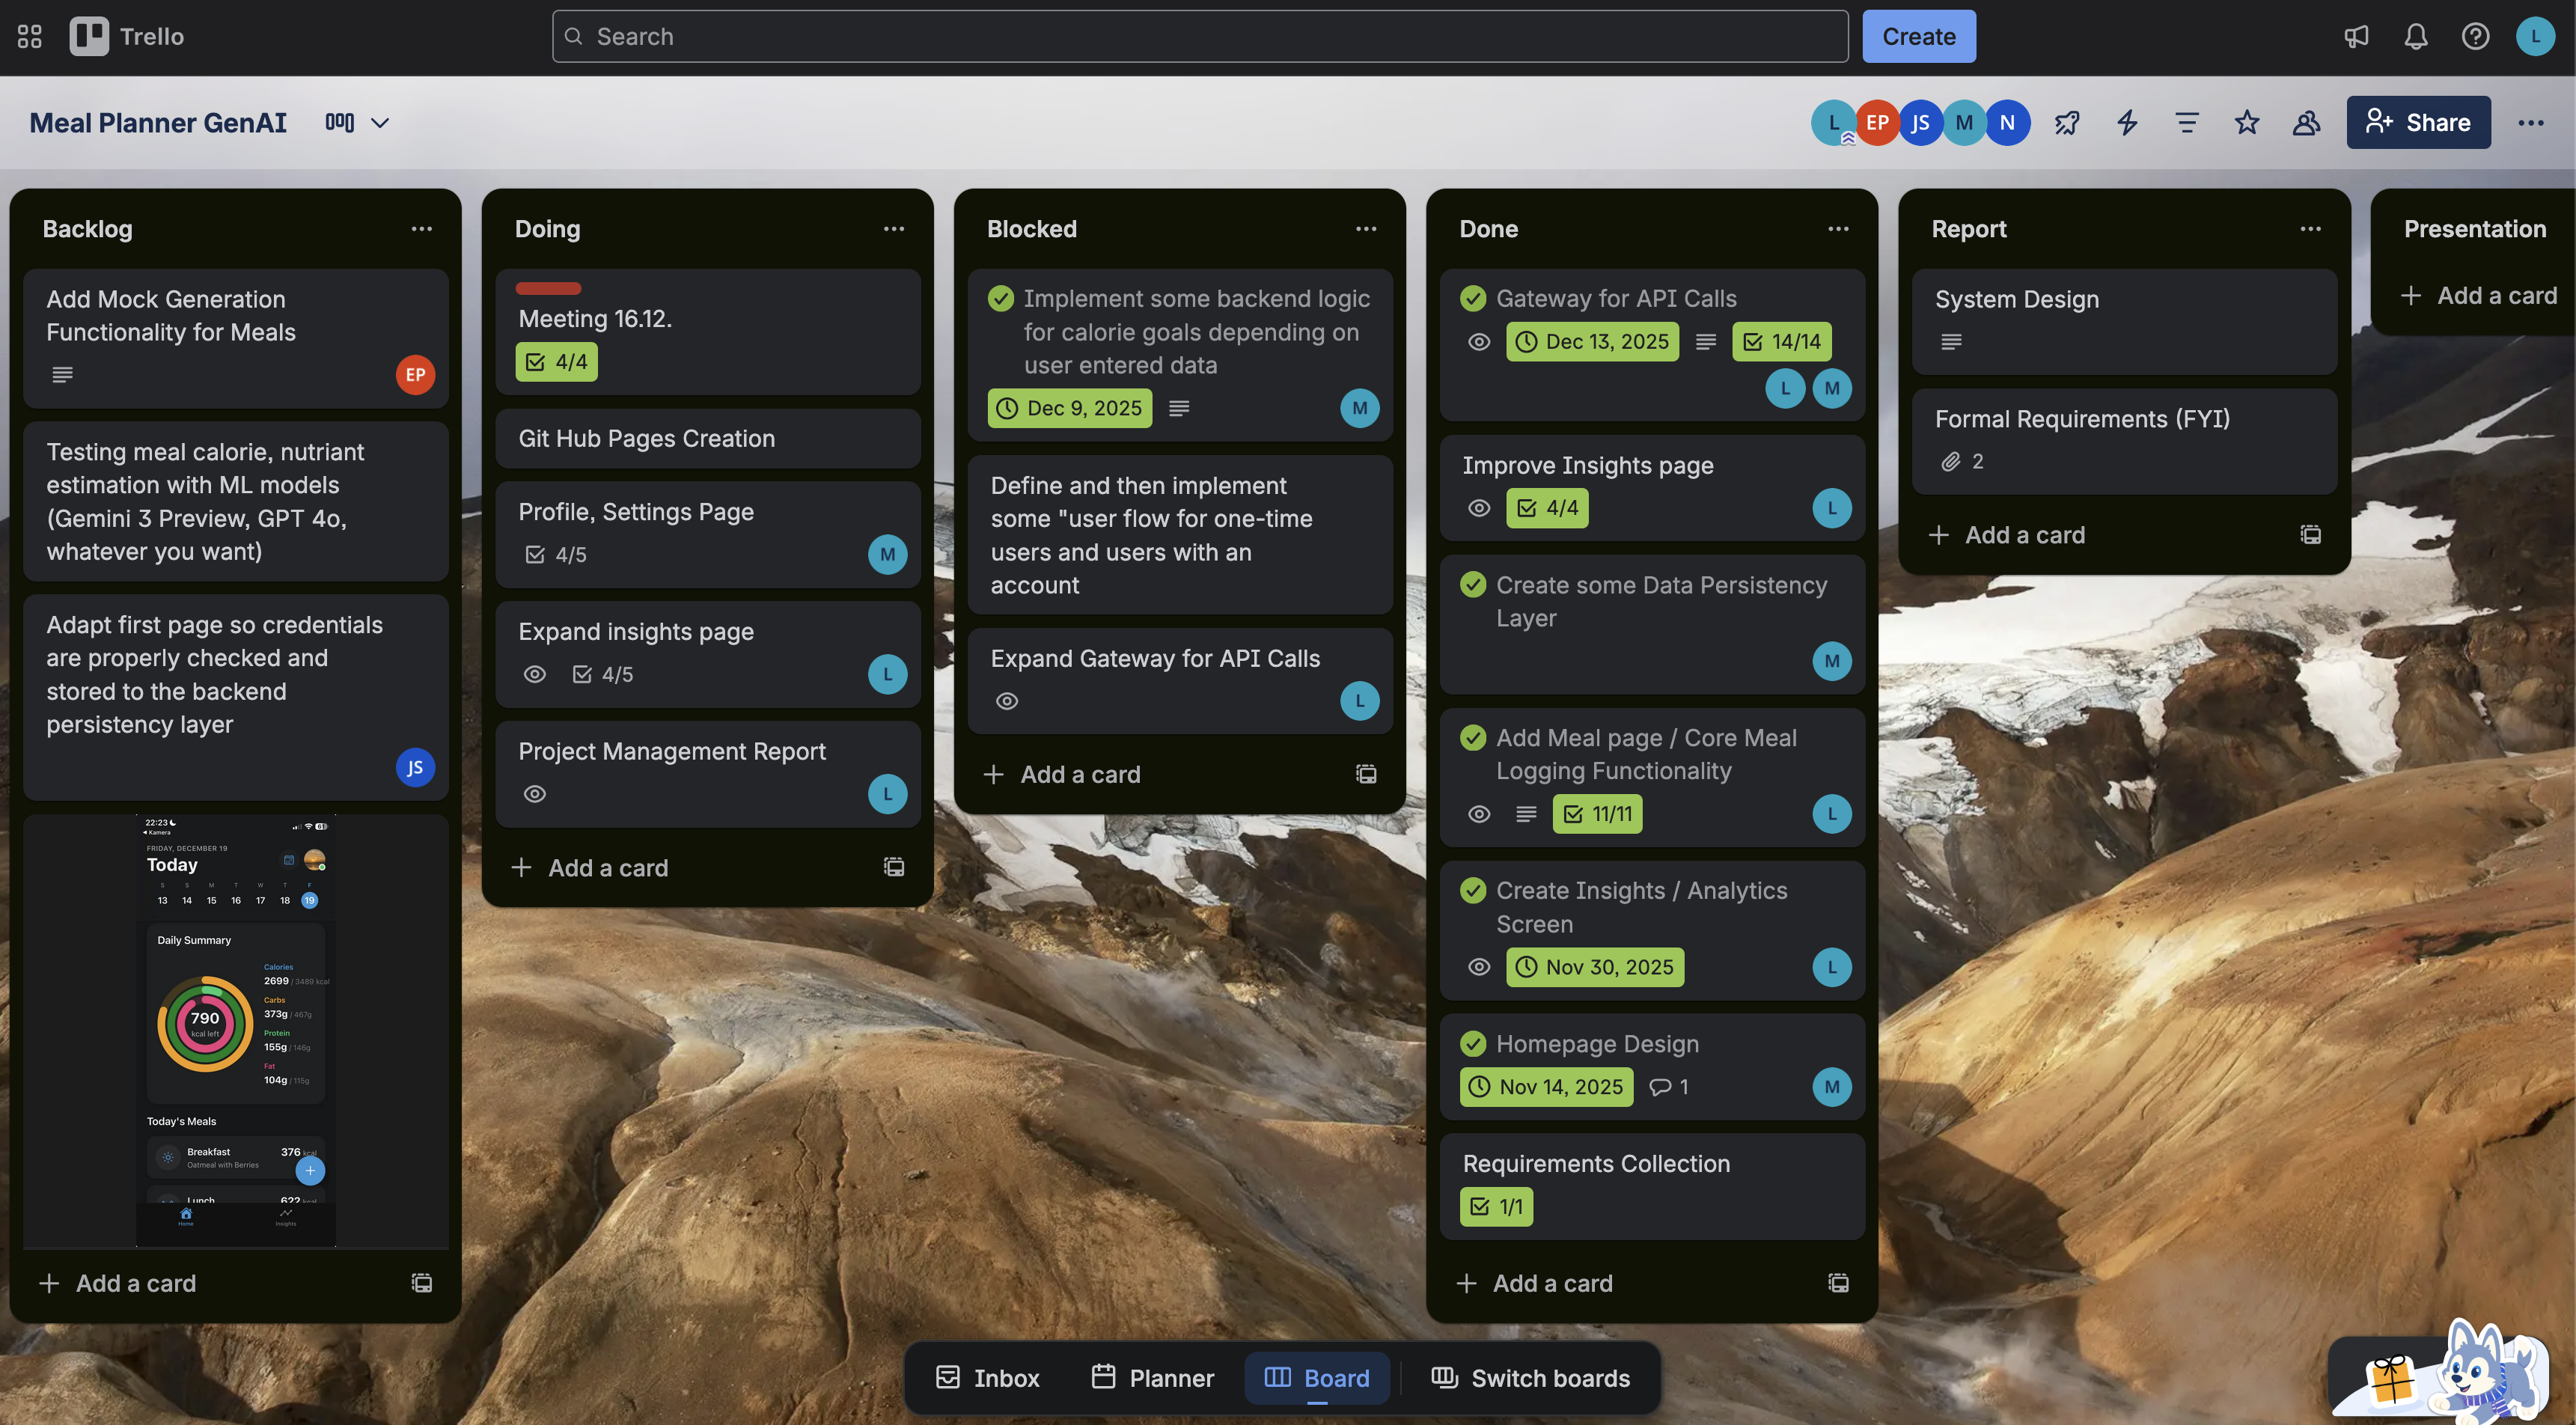
\includegraphics[width=0.8\textwidth]{trello.png}
    \caption{Project Management Board used for Development of NutriAI}
    \label{fig:trello}
    \end{center}
\end{figure}

\noindent
To keep track of the tickets and overall tasks concerning our project, we used \href{https://trello.com/}{Trello}, a project management tool that uses a flexible, Kanban-style system of boards, lists, and cards to help individuals and teams organize tasks, workflows, and ideas, making it easy to track progress from "to-do" to "done". For a screenshot taken from our project's board, refer to Figure \ref{fig:trello}.
Apart from using a project management tool, we also created a WhatsApp group with all the team members to agree on meeting dates, keep us updated and discuss immediate questions or provide advice quicklier.

\subsection{Prompt Engineering Strategies}

Key techniques used (e.g., role prompting, chain-of-thought), refinement process, and impact on GenAI performance

\section{Team roles, responsibilities, and how collaboration was managed}

\section{Current Progress and Future Plans}
Progress Status and Roadmap to Completion
Current status (completed/in-progress/pending), key achievements, risks, and final steps

\section{Project Pitch Video (Attached)}

\section{Usage of GenAI during the Document's Creation}
\noindent
Generative AI was used during the writing process to help with brainstorming and organizing initial notes.
It was also used to assist with debugging certain problems occuring with LaTeX.


\printbibliography

\end{document}
